%%%%%%%%%%%%  Generated using docx2latex.com  %%%%%%%%%%%%%%

%%%%%%%%%%%%  v2.0.0-beta  %%%%%%%%%%%%%%

\documentclass[12pt]{article}
\usepackage{amsmath}
\usepackage{latexsym}
\usepackage{amsfonts}
\usepackage[normalem]{ulem}
\usepackage{array}
\usepackage{amssymb}
\usepackage{graphicx}
\usepackage[backend=biber,
style=numeric,
sorting=none,
isbn=false,
doi=false,
url=false,
]{biblatex}\addbibresource{bibliography.bib}

\usepackage{subfig}
\usepackage{wrapfig}
\usepackage{wasysym}
\usepackage{enumitem}
\usepackage{adjustbox}
\usepackage{ragged2e}
\usepackage[svgnames,table]{xcolor}
\usepackage{tikz}
\usepackage{longtable}
\usepackage{changepage}
\usepackage{setspace}
\usepackage{hhline}
\usepackage{multicol}
\usepackage{tabto}
\usepackage{float}
\usepackage{multirow}
\usepackage{makecell}
\usepackage{fancyhdr}
\usepackage[toc,page]{appendix}
\usepackage[hidelinks]{hyperref}
\usetikzlibrary{shapes.symbols,shapes.geometric,shadows,arrows.meta}
\tikzset{>={Latex[width=1.5mm,length=2mm]}}
\usepackage{flowchart}\usepackage[paperheight=11.69in,paperwidth=8.27in,left=1.18in,right=1.18in,top=0.98in,bottom=0.98in,headheight=1in]{geometry}
\usepackage[utf8]{inputenc}
\usepackage[T1]{fontenc}
\TabPositions{0.49in,0.98in,1.47in,1.96in,2.45in,2.94in,3.43in,3.92in,4.41in,4.9in,5.39in,5.88in,}

\urlstyle{same}


 %%%%%%%%%%%%  Set Depths for Sections  %%%%%%%%%%%%%%

% 1) Section
% 1.1) SubSection
% 1.1.1) SubSubSection
% 1.1.1.1) Paragraph
% 1.1.1.1.1) Subparagraph


\setcounter{tocdepth}{5}
\setcounter{secnumdepth}{5}


 %%%%%%%%%%%%  Set Depths for Nested Lists created by \begin{enumerate}  %%%%%%%%%%%%%%


\setlistdepth{9}
\renewlist{enumerate}{enumerate}{9}
		\setlist[enumerate,1]{label=\arabic*)}
		\setlist[enumerate,2]{label=\alph*)}
		\setlist[enumerate,3]{label=(\roman*)}
		\setlist[enumerate,4]{label=(\arabic*)}
		\setlist[enumerate,5]{label=(\Alph*)}
		\setlist[enumerate,6]{label=(\Roman*)}
		\setlist[enumerate,7]{label=\arabic*}
		\setlist[enumerate,8]{label=\alph*}
		\setlist[enumerate,9]{label=\roman*}

\renewlist{itemize}{itemize}{9}
		\setlist[itemize]{label=$\cdot$}
		\setlist[itemize,1]{label=\textbullet}
		\setlist[itemize,2]{label=$\circ$}
		\setlist[itemize,3]{label=$\ast$}
		\setlist[itemize,4]{label=$\dagger$}
		\setlist[itemize,5]{label=$\triangleright$}
		\setlist[itemize,6]{label=$\bigstar$}
		\setlist[itemize,7]{label=$\blacklozenge$}
		\setlist[itemize,8]{label=$\prime$}

\setlength{\topsep}{0pt}\setlength{\parindent}{0pt}
\renewcommand{\arraystretch}{1.3}


%%%%%%%%%%%%%%%%%%%% Document code starts here %%%%%%%%%%%%%%%%%%%%



\begin{document}
\setlength{\parskip}{14.04pt}
{\fontsize{14pt}{16.8pt}\selectfont \textbf{UNIVERSIDAD POLITÉCNICA DE LA ZONA METROPOLITANA DE GUADALAJARA}\par}\par

{\fontsize{14pt}{16.8pt}\selectfont \textbf{\textcolor[HTML]{21409A}{DISEÑO DE MODULACIÓN DE ANCHO DE PULSO (PWM) CON AMP-OP Y TRANSISTORES}}\par}\par

{\fontsize{14pt}{16.8pt}\selectfont \textbf{Por: Jesús David Esparza Cabrera}\par}\par

{\fontsize{14pt}{16.8pt}\selectfont \textbf{Grado y grupo: 4-B}\par}\par



%%%%%%%%%%%%%%%%%%%% Figure/Image No: 1 starts here %%%%%%%%%%%%%%%%%%%%

\begin{figure}[H]
	\begin{Center}
		
\includegraphics[width=2.71in,height=2.74in]{./media/image1.png}
	\end{Center}
\end{figure}


%%%%%%%%%%%%%%%%%%%% Figure/Image No: 1 Ends here %%%%%%%%%%%%%%%%%%%%

\par


\vspace{\baselineskip}

\vspace{\baselineskip}

\vspace{\baselineskip}

\vspace{\baselineskip}

\vspace{\baselineskip}

\vspace{\baselineskip}

\vspace{\baselineskip}
\begin{enumerate}
	\item {\fontsize{18pt}{21.6pt}\selectfont \textcolor[HTML]{0066B3}{¿Qué es PWM?}\par}
\end{enumerate}\par

La modulación por ancho de pulso o PWM (Pulse Width Modulation) se usa para controlar el ancho de una señal digital con el propósito de controlar a su vez la potencia que se entrega a ciertos dispositivos. Modificando el ancho del pulso activo (que está en On) se controla la cantidad de corriente que fluye hacia el dispositivo.\par

\begin{enumerate}
	\item \textcolor[HTML]{0066B3}{¿Cómo funciona un PWM?}\par

Un PWM funciona como un interruptor, que constantemente se activa y desactiva, regulando la cantidad de corriente y por ende de potencia, que se entrega al dispositivo que se desea controlar. Éstos dispositivos pueden ser motores CC o fuentes de luz en CC, entre otros.\par

Si un motor es alimentado con 12 voltios, recibe todo el tiempo la corriente que este pide y entrega la máxima potencia, si es alimentado con 0 voltios, no recibe corriente y no obtiene potencia.\par

En un sistema PWM el motor recibe corriente por un tiempo y deja de recibirlo por otro, repitiéndose este proceso continuamente. Si se aumenta el tiempo en que el pulso está en nivel alto (12 V en nuestro ejemplo), se entrega más potencia y si se reduce el tiempo entrega menos potencia. Para entender mejor esta idea observar la siguiente imagen.\par



%%%%%%%%%%%%%%%%%%%% Figure/Image No: 2 starts here %%%%%%%%%%%%%%%%%%%%

\begin{figure}[H]
	\begin{Center}
		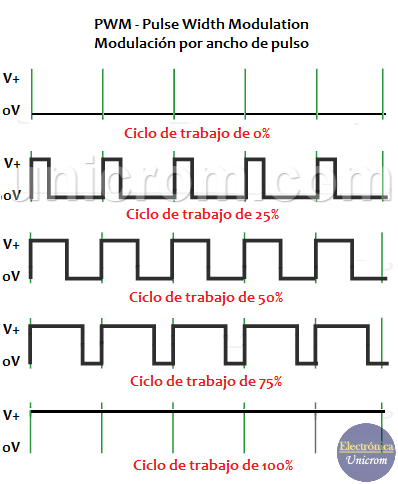
\includegraphics[width=4.15in,height=5.04in]{./media/image2.png}
	\end{Center}
\end{figure}


%%%%%%%%%%%%%%%%%%%% Figure/Image No: 2 Ends here %%%%%%%%%%%%%%%%%%%%

\par

\setlength{\parskip}{0.0pt}
\begin{itemize}
	\item Si el ciclo de trabajo es de 0$\%$  significa que no hay tiempo con pulso en nivel alto y el motor está apagado. \par

	\item Si el ciclo de trabajo es de 25$\%$  significa que el 25$\%$  del tiempo el pulso está en nivel alto y el 75$\%$  en nivel bajo. \par

	\item Si el ciclo de trabajo es de 50$\%$  el tiempo que el voltaje está en bajo es igual al que está en alto. \par

	\item Si el ciclo de trabajo es de 100$\%$ , significa que el pulso está todo el tiempo en nivel alto. Esto causa que el motor esté trabajando al máximo porque recibe corriente todo el tiempo. 
\end{itemize}\par

\begin{enumerate}
	\item \textcolor[HTML]{0066B3}{¿Qué ventajas tiene la modulación por ancho de pulso?}\par

La principal ventaja es la eficiencia energética. El circuito que tenga este método de control, entrega a la carga una cantidad de potencia que es proporcional a la potencia que necesita para realizar su trabajo.\par

\begin{itemize}
	\item Si se necesita aumentar la velocidad de un motor se incrementa la potencia que se le entrega (ciclo de trabajo mayor) \par

	\item Si se necesita disminuir la velocidad de un motor se disminuye la potencia que se le entrega. (ciclo de trabajo menor) 
\end{itemize}\par

	\item \textcolor[HTML]{0066B3}{¿Qué aplicaciones tiene el PWM?}\par

\begin{itemize}
	\item Controles de velocidad variables para motores CC \par

	\item Dimmers para sistemas de iluminación con LEDs 
\end{itemize}\par

	\item \textcolor[HTML]{0066B3}{Ejemplo de aplicación de la modulación por ancho de pulso.}
\end{enumerate}\par

	\item \textcolor[HTML]{0066B3}{Control de la intensidad de iluminación de unos LEDs.}\par



%%%%%%%%%%%%%%%%%%%% Figure/Image No: 3 starts here %%%%%%%%%%%%%%%%%%%%

\begin{figure}[H]
	\begin{Center}
		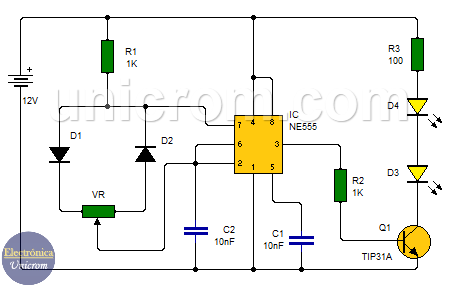
\includegraphics[width=4.75in,height=2.99in]{./media/image3.png}
	\end{Center}
\end{figure}


%%%%%%%%%%%%%%%%%%%% Figure/Image No: 3 Ends here %%%%%%%%%%%%%%%%%%%%

\par


\vspace{\baselineskip}

\end{enumerate}
\vspace{\baselineskip}

\vspace{\baselineskip}
Éste circuito utiliza el conocido temporizador 555. Éste circuito integrado es conectado como multivibrador astable, y entrega en su salida una onda cuadrada.\par

El ciclo de trabajo de la onda de salida se controla con el potenciómetro, el transistor se encarga de activar y desactivar la carga (en este caso dos LEDs), según el ciclo de trabajo.\par

Modificando el ciclo de trabajo se puede pasar de apagado total (ciclo del 0$\%$ ) a encendido total (ciclo del 100$\%$ ). Si se desea una intensidad de luz intermedia se puede utilizar un ciclo del 50$\%$  o un porcentaje cercano.\par

De la misma manera también se puede controlar la velocidad del motor CC.\par

\begin{enumerate}
	\item \begin{enumerate}
	\item \begin{enumerate}
	\item \textcolor[HTML]{0066B3}{Control de velocidad de un motor CC}
\end{enumerate}
\end{enumerate}
\end{enumerate}\par

El siguiente circuito es igual al anterior, pero se han cambiado los LED y la resistencia de 100 ohmios  por un motor CC con un diodo en paralelo pero invertido, con el propósito de proteger el transistor.\par



%%%%%%%%%%%%%%%%%%%% Figure/Image No: 4 starts here %%%%%%%%%%%%%%%%%%%%

\begin{figure}[H]
	\begin{Center}
		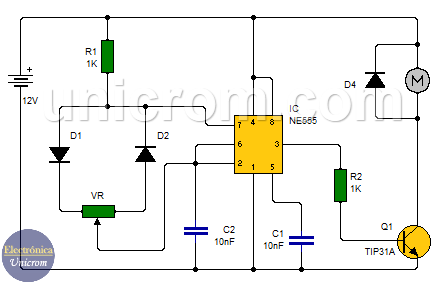
\includegraphics[width=4.62in,height=2.96in]{./media/image4.png}
	\end{Center}
\end{figure}


%%%%%%%%%%%%%%%%%%%% Figure/Image No: 4 Ends here %%%%%%%%%%%%%%%%%%%%

\par

La velocidad del motor CC cambiará con la variación del ciclo de trabajo escogido con el potenciómetro.\par

Para amplificaciones en corriente alterna, se puede optar por un \href{https://unicrom.com/dimmer-control-de-velocidad-motor-ac-con-triac/}{dimmer o control de velocidad de motores en CA/AC}. \par


\vspace{\baselineskip}
{\fontsize{18pt}{21.6pt}\selectfont \textbf{\textcolor[HTML]{0066B3}{Bibliografía:}}\par}\par

\href{https://bibdigital.epn.edu.ec/bitstream/15000/10695/1/T1493.pdf}{\textbf{\textcolor[HTML]{BD7CB5}{https://bibdigital.epn.edu.ec › bitstream}}}\par


\vspace{\baselineskip}

\vspace{\baselineskip}

\vspace{\baselineskip}
\setlength{\parskip}{14.04pt}

\vspace{\baselineskip}

\vspace{\baselineskip}

\vspace{\baselineskip}

\vspace{\baselineskip}

\vspace{\baselineskip}

\vspace{\baselineskip}

\vspace{\baselineskip}

\vspace{\baselineskip}

\vspace{\baselineskip}

\vspace{\baselineskip}

\vspace{\baselineskip}

\vspace{\baselineskip}

\vspace{\baselineskip}

\vspace{\baselineskip}

\vspace{\baselineskip}

\vspace{\baselineskip}

\vspace{\baselineskip}

\vspace{\baselineskip}

\vspace{\baselineskip}

\vspace{\baselineskip}

\vspace{\baselineskip}

\vspace{\baselineskip}

\vspace{\baselineskip}

\vspace{\baselineskip}

\vspace{\baselineskip}

\vspace{\baselineskip}

\vspace{\baselineskip}

\vspace{\baselineskip}

\vspace{\baselineskip}

\vspace{\baselineskip}

\vspace{\baselineskip}

\vspace{\baselineskip}

\vspace{\baselineskip}

\vspace{\baselineskip}

\vspace{\baselineskip}

\vspace{\baselineskip}

\vspace{\baselineskip}

\vspace{\baselineskip}

\vspace{\baselineskip}

\vspace{\baselineskip}

\vspace{\baselineskip}

\vspace{\baselineskip}

\vspace{\baselineskip}
{\fontsize{15pt}{18.0pt}\selectfont \textbf{Bibliografía}\par}\par

\href{http://perso.wanadoo.es/luis_ju/ebasica2/mcc_01.html}{http://perso.wanadoo.es/luis\_ju/ebasica2/mcc\_01.html}\par

\setlength{\parskip}{6.96pt}
\href{http://www.unicrom.com/Tut_MotorCC.asp}{http://www.unicrom.com/Tut\_MotorCC.asp}\par


\printbibliography
\end{document}